\documentclass[8pt,aspectratio=169]{beamer}
\usetheme{Madrid}
\usepackage{graphicx}
\usepackage{booktabs}
\usepackage{adjustbox}
\usepackage{multicol}
\usepackage{amsmath}
\usepackage{listings}
\usepackage{tikz}
\usetikzlibrary{shapes,arrows,positioning,calc,fit}

% Color definitions
\definecolor{mlblue}{RGB}{0,102,204}
\definecolor{mlpurple}{RGB}{51,51,178}
\definecolor{mllavender}{RGB}{173,173,224}
\definecolor{mllavender2}{RGB}{193,193,232}
\definecolor{mllavender3}{RGB}{204,204,235}
\definecolor{mllavender4}{RGB}{214,214,239}
\definecolor{mlorange}{RGB}{255, 127, 14}
\definecolor{mlgreen}{RGB}{44, 160, 44}
\definecolor{mlred}{RGB}{214, 39, 40}
\definecolor{mlgray}{RGB}{127, 127, 127}

% Additional colors for template compatibility
\definecolor{lightgray}{RGB}{240, 240, 240}
\definecolor{midgray}{RGB}{180, 180, 180}

% Solidity code colors
\definecolor{solkeyword}{RGB}{0, 102, 153}
\definecolor{solstring}{RGB}{163, 21, 21}
\definecolor{solcomment}{RGB}{0, 128, 0}
\definecolor{solnumber}{RGB}{0, 128, 128}

% Apply custom colors to Madrid theme
\setbeamercolor{palette primary}{bg=mllavender3,fg=mlpurple}
\setbeamercolor{palette secondary}{bg=mllavender2,fg=mlpurple}
\setbeamercolor{palette tertiary}{bg=mllavender,fg=white}
\setbeamercolor{palette quaternary}{bg=mlpurple,fg=white}

\setbeamercolor{structure}{fg=mlpurple}
\setbeamercolor{section in toc}{fg=mlpurple}
\setbeamercolor{subsection in toc}{fg=mlblue}
\setbeamercolor{title}{fg=mlpurple}
\setbeamercolor{frametitle}{fg=mlpurple,bg=mllavender3}
\setbeamercolor{block title}{bg=mllavender2,fg=mlpurple}
\setbeamercolor{block body}{bg=mllavender4,fg=black}

% Remove navigation symbols
\setbeamertemplate{navigation symbols}{}

% Clean itemize/enumerate
\setbeamertemplate{itemize items}[circle]
\setbeamertemplate{enumerate items}[default]

% Reduce margins for more content space
\setbeamersize{text margin left=5mm,text margin right=5mm}

% Listings configuration for Solidity
\lstdefinelanguage{Solidity}{
  keywords={pragma, solidity, contract, function, public, private, external, internal, view, pure, payable, returns, return, if, else, for, while, mapping, address, uint, uint256, int, string, bool, bytes, bytes32, event, emit, modifier, require, constructor, memory, storage, calldata, msg, sender, value, this, new, delete, true, false},
  keywordstyle=\color{solkeyword}\bfseries,
  ndkeywords={},
  ndkeywordstyle=\color{mlblue}\bfseries,
  sensitive=true,
  comment=[l]{//},
  morecomment=[s]{/*}{*/},
  commentstyle=\color{solcomment}\ttfamily,
  stringstyle=\color{solstring}\ttfamily,
  morestring=[b]',
  morestring=[b]"
}

\lstset{
  language=Solidity,
  basicstyle=\ttfamily\scriptsize,
  breaklines=true,
  frame=single,
  backgroundcolor=\color{lightgray},
  numbers=left,
  numberstyle=\tiny\color{mlgray},
  numbersep=5pt,
  tabsize=2,
  showstringspaces=false
}

% Python listings
\lstdefinestyle{python}{
  language=Python,
  basicstyle=\ttfamily\scriptsize,
  keywordstyle=\color{solkeyword}\bfseries,
  stringstyle=\color{solstring},
  commentstyle=\color{solcomment},
  breaklines=true,
  frame=single,
  backgroundcolor=\color{lightgray},
  numbers=left,
  numberstyle=\tiny\color{mlgray},
  numbersep=5pt,
  tabsize=2,
  showstringspaces=false
}

% JavaScript listings
\lstdefinestyle{javascript}{
  language=Java,
  basicstyle=\ttfamily\scriptsize,
  keywordstyle=\color{solkeyword}\bfseries,
  stringstyle=\color{solstring},
  commentstyle=\color{solcomment},
  morekeywords={async, await, const, let, require, describe, it, before, deploy, ethers},
  breaklines=true,
  frame=single,
  backgroundcolor=\color{lightgray},
  numbers=left,
  numberstyle=\tiny\color{mlgray},
  numbersep=5pt,
  tabsize=2,
  showstringspaces=false
}

% Command for bottom annotation (Madrid-style)
\newcommand{\bottomnote}[1]{%
\vfill
\vspace{-2mm}
\textcolor{mllavender2}{\rule{\textwidth}{0.4pt}}
\vspace{1mm}
\footnotesize
\textbf{#1}
}

\title{Ethereum \& Smart Contracts}
\subtitle{Lesson 3 of 4: Cryptocurrency Course}
\author{Prof. Dr. Joerg Osterrieder}
\institute{Academic Presentation}
\date{\today}

\begin{document}

% ==================== SLIDE 1: TITLE ====================
\begin{frame}[plain]
\vspace{2cm}
\begin{center}
{\Huge Ethereum \& Smart Contracts}\\[0.5cm]
{\Large Lesson 3 of 4: Cryptocurrency Course}\\[1.5cm]
{\normalsize Building Programmable Money}\\[0.5cm]
{\small From Bitcoin's Digital Gold to Ethereum's World Computer}
\end{center}
\end{frame}

% ==================== SLIDE 2: PREREQUISITES ====================
\begin{frame}{Prerequisites}
\textbf{Before this lesson, you should understand:}
\begin{itemize}
\item Lessons 1-2: Blockchain fundamentals and cryptography
\item Basic programming concepts (functions, variables, loops)
\item How to use a command-line interface
\end{itemize}

\vspace{1em}
\textbf{Software needed:}
\begin{itemize}
\item Node.js v18+ (\texttt{nodejs.org})
\item Hardhat development environment (\texttt{npm install --save-dev hardhat})
\item MetaMask browser extension (optional, for testnet)
\item VS Code with Solidity extension (recommended)
\end{itemize}

\vspace{1em}
\textbf{What you'll build:}\\
Your first smart contract on Ethereum!

\bottomnote{This lesson transitions from theory to hands-on smart contract development.}
\end{frame}

% ==================== SLIDE 3: OUTLINE ====================
\begin{frame}[t]{Lesson Outline}
\tableofcontents
\vfill
\footnotesize
\textbf{Duration:} 45 minutes | \textbf{Slides:} 30 | \textbf{Goal:} Understand Ethereum architecture, gas mechanics, and write your first smart contract
\end{frame}

% ==================== SECTION 1: ETHEREUM VS BITCOIN ====================
\section{Ethereum vs Bitcoin}

\begin{frame}[t]
\vfill
\centering
\begin{beamercolorbox}[sep=8pt,center]{title}
\usebeamerfont{title}\Large Section 1: Ethereum vs Bitcoin\par
\end{beamercolorbox}
\vfill
\small \textit{8 minutes}
\end{frame}

% ==================== SLIDE 3: BITCOIN - DIGITAL GOLD ====================
\begin{frame}[t]{Bitcoin: Digital Gold with Simple Scripts}
\begin{columns}[T]
\column{0.48\textwidth}
\textbf{Bitcoin's Design Philosophy}

\begin{itemize}
\item \textbf{Purpose:} Store of value, peer-to-peer cash
\item \textbf{Script:} Intentionally limited (non-Turing complete)
\item \textbf{Operations:} Basic conditions for spending
\end{itemize}

\vspace{0.5em}
\textbf{Bitcoin Script Capabilities}
\begin{itemize}
\item Multi-signature transactions
\item Time-locked transactions (CLTV, CSV)
\item Hash locks (HTLCs for Lightning)
\item Simple conditional logic
\end{itemize}

\column{0.48\textwidth}
\textbf{Why Limited by Design?}

\begin{itemize}
\item[\textcolor{mlgreen}{+}] Security through simplicity
\item[\textcolor{mlgreen}{+}] Predictable execution
\item[\textcolor{mlgreen}{+}] No infinite loops possible
\item[\textcolor{mlgreen}{+}] Smaller attack surface
\end{itemize}

\vspace{0.5em}
\textbf{Limitations}
\begin{itemize}
\item[\textcolor{mlorange}{-}] No loops or complex logic
\item[\textcolor{mlorange}{-}] No state storage
\item[\textcolor{mlorange}{-}] Limited programmability
\item[\textcolor{mlorange}{-}] Can't build complex apps
\end{itemize}
\end{columns}

\bottomnote{Bitcoin Script: Stack-based, ~100 opcodes, designed for transaction validation only}
\end{frame}

% ==================== SLIDE 4: ETHEREUM - WORLD COMPUTER ====================
\begin{frame}[t]{Ethereum: The World Computer}
\begin{columns}[T]
\column{0.48\textwidth}
\textbf{Ethereum's Vision (Vitalik Buterin, 2014)}

A blockchain with a \textbf{Turing-complete} programming language enabling:

\begin{itemize}
\item Arbitrary computation on-chain
\item Self-executing contracts
\item Decentralized applications (dApps)
\item Programmable money and assets
\end{itemize}

\vspace{0.5em}
\textbf{Key Innovation}
\begin{itemize}
\item State stored on blockchain
\item Code lives on-chain permanently
\item Anyone can interact with contracts
\item Trustless execution guaranteed
\end{itemize}

\column{0.48\textwidth}
\textbf{Comparison: Bitcoin vs Ethereum}

\begin{center}
\begin{tabular}{lcc}
\toprule
\textbf{Feature} & \textbf{BTC} & \textbf{ETH} \\
\midrule
Purpose & Currency & Platform \\
Scripts & Limited & Full \\
State & UTXO & Account \\
Loops & No & Yes \\
Storage & No & Yes \\
Gas & No & Yes \\
\bottomrule
\end{tabular}
\end{center}

\vspace{0.5em}
\textbf{Result:} DeFi, NFTs, DAOs, Tokens
\end{columns}

\bottomnote{Turing-complete: Can compute anything computable given enough resources}
\end{frame}

% ==================== SLIDE 5: ETHEREUM ARCHITECTURE CHART ====================
\begin{frame}[t]{Ethereum Architecture Overview}
\begin{center}
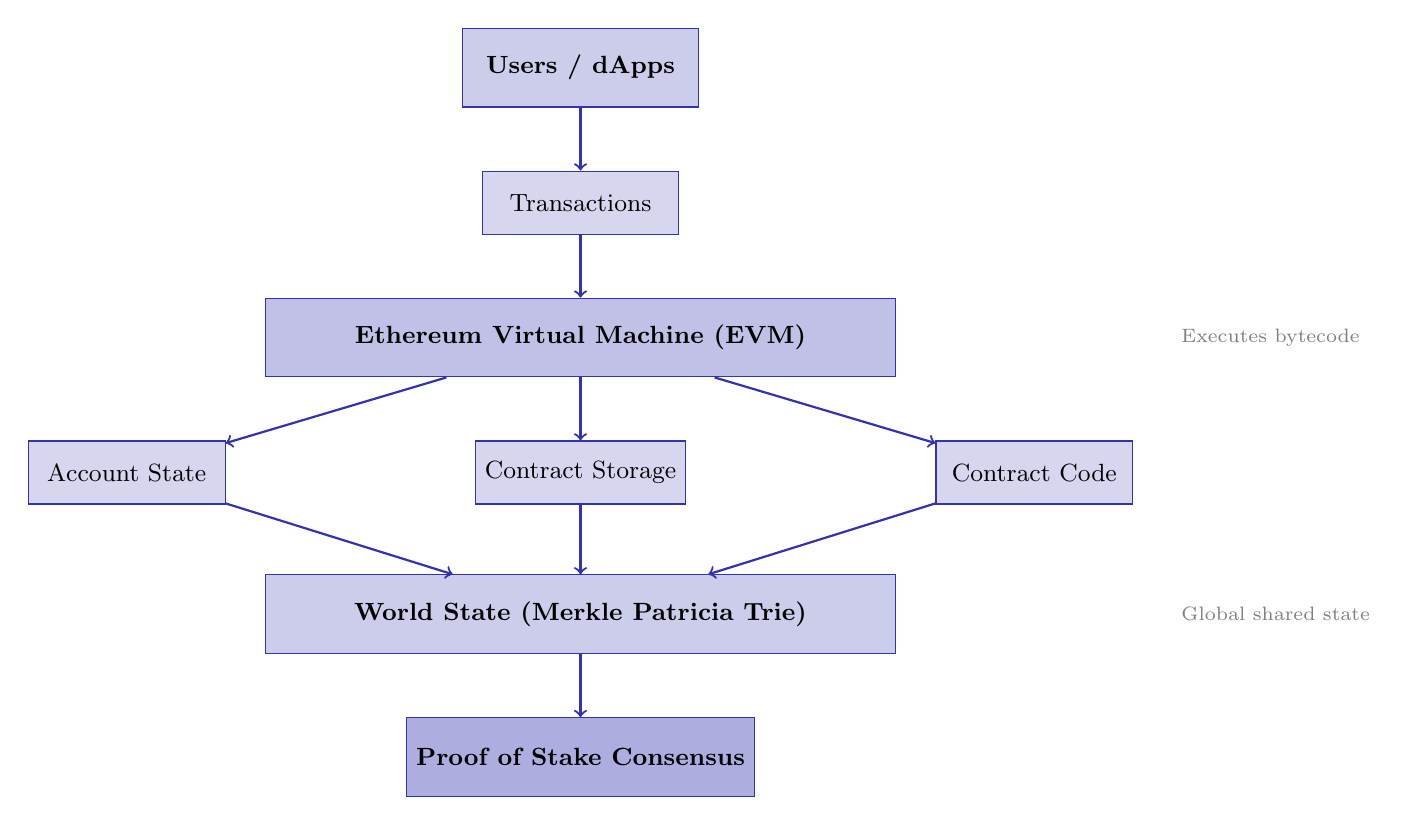
\begin{tikzpicture}[
  node distance=0.8cm,
  box/.style={rectangle, draw=mlpurple, fill=mllavender4, minimum width=2.5cm, minimum height=0.8cm, align=center, font=\small},
  bigbox/.style={rectangle, draw=mlpurple, fill=mllavender3, minimum width=3cm, minimum height=1cm, align=center, font=\small\bfseries},
  arrow/.style={->, thick, mlpurple}
]

% Layer 1 - Users
\node[bigbox] (users) {Users / dApps};

% Layer 2 - Transactions
\node[box, below=of users] (tx) {Transactions};

% Layer 3 - EVM
\node[bigbox, below=of tx, minimum width=8cm, fill=mllavender2] (evm) {Ethereum Virtual Machine (EVM)};

% Layer 4 - State components
\node[box, below left=0.8cm and 0.5cm of evm] (accounts) {Account State};
\node[box, below=0.8cm of evm] (storage) {Contract Storage};
\node[box, below right=0.8cm and 0.5cm of evm] (code) {Contract Code};

% Layer 5 - World State
\node[bigbox, below=2.5cm of evm, minimum width=8cm] (state) {World State (Merkle Patricia Trie)};

% Layer 6 - Consensus
\node[bigbox, below=of state, fill=mllavender] (consensus) {Proof of Stake Consensus};

% Arrows
\draw[arrow] (users) -- (tx);
\draw[arrow] (tx) -- (evm);
\draw[arrow] (evm) -- (accounts);
\draw[arrow] (evm) -- (storage);
\draw[arrow] (evm) -- (code);
\draw[arrow] (accounts) -- (state);
\draw[arrow] (storage) -- (state);
\draw[arrow] (code) -- (state);
\draw[arrow] (state) -- (consensus);

% Labels
\node[right=3.5cm of evm, font=\scriptsize, text=mlgray] {Executes bytecode};
\node[right=3.5cm of state, font=\scriptsize, text=mlgray] {Global shared state};

\end{tikzpicture}
\end{center}

\bottomnote{Every node maintains identical state; EVM ensures deterministic execution across all nodes}
\end{frame}

% ==================== SLIDE 6: THE EVM EXPLAINED ====================
\begin{frame}[t]{The Ethereum Virtual Machine (EVM)}
\begin{columns}[T]
\column{0.48\textwidth}
\textbf{What is the EVM?}

A \textbf{stack-based virtual machine} that:
\begin{itemize}
\item Executes smart contract bytecode
\item Runs identically on every node
\item Ensures deterministic results
\item Meters computation with gas
\end{itemize}

\vspace{0.5em}
\textbf{EVM Characteristics}
\begin{itemize}
\item 256-bit word size (for crypto ops)
\item 1024 stack depth limit
\item Memory: byte-addressable, volatile
\item Storage: 256-bit to 256-bit mapping
\end{itemize}

\column{0.48\textwidth}
\textbf{EVM Execution Model}

\begin{center}
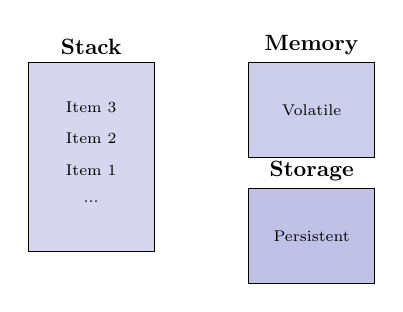
\begin{tikzpicture}[scale=0.8, every node/.style={scale=0.8}]
  \node[draw, rectangle, fill=mllavender4, minimum width=2cm, minimum height=3cm] (stack) at (0,0) {};
  \node[above] at (stack.north) {\textbf{Stack}};
  \node at (0,0.8) {\scriptsize Item 3};
  \node at (0,0.3) {\scriptsize Item 2};
  \node at (0,-0.2) {\scriptsize Item 1};
  \node at (0,-0.7) {\scriptsize ...};

  \node[draw, rectangle, fill=mllavender3, minimum width=2cm, minimum height=1.5cm] (mem) at (3.5,0.75) {};
  \node[above] at (mem.north) {\textbf{Memory}};
  \node at (3.5,0.75) {\scriptsize Volatile};

  \node[draw, rectangle, fill=mllavender2, minimum width=2cm, minimum height=1.5cm] (stor) at (3.5,-1.25) {};
  \node[above] at (stor.north) {\textbf{Storage}};
  \node at (3.5,-1.25) {\scriptsize Persistent};
\end{tikzpicture}
\end{center}

\textbf{Opcodes:} ADD, MUL, SLOAD, SSTORE, CALL, CREATE, SELFDESTRUCT, etc.
\end{columns}

\bottomnote{EVM bytecode is compiled from high-level languages like Solidity, Vyper, or Yul}
\end{frame}

% ==================== SLIDE 7: ACCOUNTS - EOA VS CONTRACT ====================
\begin{frame}[t]{Ethereum Accounts: EOA vs Contract}
\begin{columns}[T]
\column{0.48\textwidth}
\textbf{Externally Owned Accounts (EOA)}

Controlled by private keys (humans/wallets):

\begin{itemize}
\item Has ETH balance
\item Can send transactions
\item No code associated
\item Address from public key hash
\item Signs transactions with private key
\end{itemize}

\vspace{0.5em}
\textbf{Account State}
\begin{itemize}
\item \texttt{nonce}: Transaction count
\item \texttt{balance}: ETH in Wei
\end{itemize}

\column{0.48\textwidth}
\textbf{Contract Accounts}

Controlled by code (autonomous):

\begin{itemize}
\item Has ETH balance
\item Has associated code
\item Has persistent storage
\item Address from creator + nonce
\item Executes when triggered
\end{itemize}

\vspace{0.5em}
\textbf{Additional State}
\begin{itemize}
\item \texttt{codeHash}: Hash of bytecode
\item \texttt{storageRoot}: Merkle root of storage
\end{itemize}
\end{columns}

\vspace{0.5em}
\begin{center}
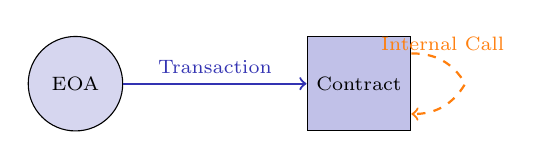
\begin{tikzpicture}[scale=0.9]
  \node[draw, circle, fill=mllavender4, minimum size=1.2cm] (eoa) at (0,0) {\scriptsize EOA};
  \node[draw, rectangle, fill=mllavender2, minimum size=1.2cm] (contract) at (4,0) {\scriptsize Contract};
  \draw[->, thick, mlpurple] (eoa) -- node[above, font=\scriptsize] {Transaction} (contract);
  \draw[->, thick, mlorange, dashed] (contract) to[bend left=30] node[above, font=\scriptsize] {Internal Call} (5.5,0) to[bend left=30] (contract);
\end{tikzpicture}
\end{center}

\bottomnote{Only EOAs can initiate transactions; contracts react to calls}
\end{frame}

% ==================== SECTION 2: GAS & TRANSACTIONS ====================
\section{Gas \& Transactions}

\begin{frame}[t]
\vfill
\centering
\begin{beamercolorbox}[sep=8pt,center]{title}
\usebeamerfont{title}\Large Section 2: Gas \& Transactions\par
\end{beamercolorbox}
\vfill
\small \textit{7 minutes}
\end{frame}

% ==================== SLIDE 8: WHAT IS GAS? ====================
\begin{frame}[t]{What is Gas?}
\begin{columns}[T]
\column{0.48\textwidth}
\textbf{Gas = Computational Fuel}

\begin{itemize}
\item Unit measuring computational work
\item Every operation costs gas
\item Paid in ETH (gas price x gas used)
\item Prevents infinite loops
\item Incentivizes efficient code
\end{itemize}

\vspace{0.3em}
\begin{block}{Real-World Analogy}
Gas is like \textbf{postage stamps for letters}. A simple letter (basic transaction) needs one stamp. A heavy package (complex smart contract) needs more stamps. The heavier your package, the more you pay!
\end{block}

\vspace{0.3em}
\textbf{Why Not Just Use ETH?}
\begin{itemize}
\item Decouples computation cost from ETH price
\item Gas costs stay stable in gas units
\item Price adjusts via market (gas price)
\end{itemize}

\column{0.48\textwidth}
\textbf{Gas Costs (Examples)}

\begin{center}
\begin{tabular}{lr}
\toprule
\textbf{Operation} & \textbf{Gas} \\
\midrule
ADD/SUB & 3 \\
MUL/DIV & 5 \\
SLOAD (storage read) & 2,100 \\
SSTORE (new value) & 20,000 \\
SSTORE (update) & 5,000 \\
CREATE (contract) & 32,000 \\
Transaction base & 21,000 \\
\bottomrule
\end{tabular}
\end{center}

\vspace{0.3em}
\textit{Storage is expensive by design!}
\end{columns}

\bottomnote{Gas prevents spam and DoS attacks; miners/validators prioritize higher-paying transactions}
\end{frame}

% ==================== SLIDE 9: GAS = EXECUTION COST ====================
\begin{frame}[t]{Gas Economics: Execution Cost}
\begin{columns}[T]
\column{0.48\textwidth}
\textbf{Transaction Fee Calculation}

$$\text{Fee} = \text{Gas Used} \times \text{Gas Price}$$

\vspace{0.5em}
\textbf{Example Transaction}
\begin{itemize}
\item Gas Used: 50,000 gas
\item Gas Price: 30 Gwei
\item Fee: $50{,}000 \times 30 = 1{,}500{,}000$ Gwei
\item Fee: $0.0015$ ETH
\item At \$2000/ETH: \$3.00
\end{itemize}

\vspace{0.5em}
\textbf{Unit Conversions}
\begin{itemize}
\item 1 ETH = $10^{18}$ Wei
\item 1 Gwei = $10^{9}$ Wei
\item 1 ETH = $10^{9}$ Gwei
\end{itemize}

\column{0.48\textwidth}
\textbf{EIP-1559 Fee Structure (Post-London)}

\begin{itemize}
\item \textbf{Base Fee:} Algorithmically set, burned
\item \textbf{Priority Fee (Tip):} Goes to validator
\item \textbf{Max Fee:} User's maximum willing to pay
\end{itemize}

$$\text{Fee} = \text{Gas} \times (\text{Base} + \text{Tip})$$

\vspace{0.5em}
\textbf{Benefits of EIP-1559}
\begin{itemize}
\item More predictable fees
\item ETH becomes deflationary (burning)
\item Better UX for fee estimation
\end{itemize}
\end{columns}

\bottomnote{Average transaction: 21,000 gas (transfer) to 500,000+ gas (complex contract interaction)}
\end{frame}

% ==================== SLIDE 10: GAS MECHANICS CHART ====================
\begin{frame}[t]{Gas Mechanics Visualization}
\begin{center}
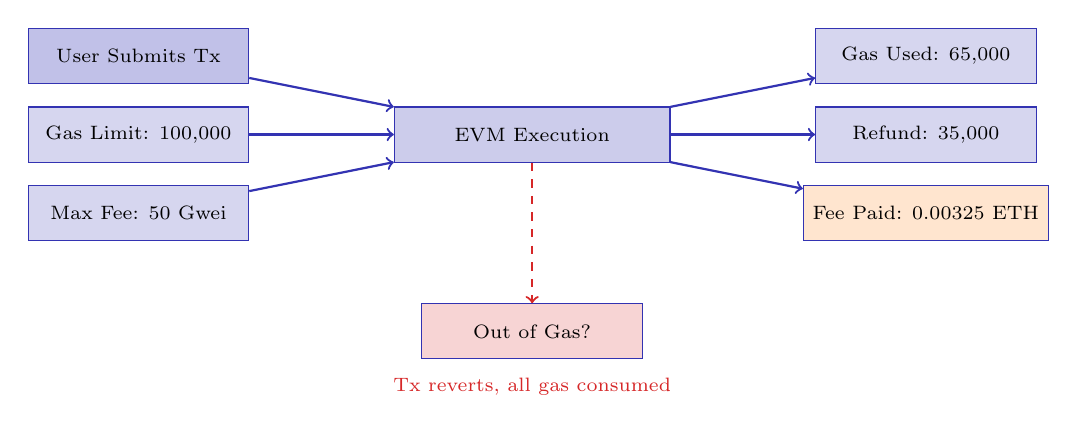
\begin{tikzpicture}[
  node distance=0.6cm,
  box/.style={rectangle, draw=mlpurple, fill=mllavender4, minimum width=2.8cm, minimum height=0.7cm, align=center, font=\scriptsize},
  arrow/.style={->, thick, mlpurple}
]

% Transaction flow
\node[box, fill=mllavender2] (user) at (0,3) {User Submits Tx};
\node[box] (limit) at (0,2) {Gas Limit: 100,000};
\node[box] (price) at (0,1) {Max Fee: 50 Gwei};

\node[box, fill=mllavender3, minimum width=3.5cm] (evm) at (5,2) {EVM Execution};

\node[box] (used) at (10,3) {Gas Used: 65,000};
\node[box] (refund) at (10,2) {Refund: 35,000};
\node[box, fill=mlorange!20] (fee) at (10,1) {Fee Paid: 0.00325 ETH};

% Arrows
\draw[arrow] (user) -- (evm);
\draw[arrow] (limit) -- (evm);
\draw[arrow] (price) -- (evm);
\draw[arrow] (evm) -- (used);
\draw[arrow] (evm) -- (refund);
\draw[arrow] (evm) -- (fee);

% Out of gas scenario
\node[box, fill=mlred!20] (oog) at (5,-0.5) {Out of Gas?};
\node[font=\scriptsize, text=mlred] at (5,-1.2) {Tx reverts, all gas consumed};

\draw[arrow, mlred, dashed] (evm) -- (oog);

\end{tikzpicture}
\end{center}

\vspace{0.5em}
\begin{columns}[T]
\column{0.48\textwidth}
\textbf{Success Scenario}
\begin{itemize}
\item Execution completes within limit
\item Unused gas refunded to sender
\item State changes persisted
\end{itemize}

\column{0.48\textwidth}
\textbf{Out of Gas Scenario}
\begin{itemize}
\item Execution halts at limit
\item ALL gas consumed (no refund)
\item State changes reverted
\end{itemize}
\end{columns}

\bottomnote{Always estimate gas before sending; tools like Hardhat provide accurate estimates}
\end{frame}

% ==================== SLIDE 11: GAS PRICE, LIMIT, FEE ====================
\begin{frame}[t]{Gas Components: Price, Limit, and Fees}
\begin{columns}[T]
\column{0.32\textwidth}
\textbf{Gas Limit}

Maximum gas you authorize:
\begin{itemize}
\item Set by transaction sender
\item Protects from runaway costs
\item Too low = transaction fails
\item Block gas limit: ~30M
\end{itemize}

\vspace{0.3em}
\textit{Tip: Use 20-50\% buffer}

\column{0.32\textwidth}
\textbf{Gas Price}

How much you pay per gas unit:
\begin{itemize}
\item Market-driven (supply/demand)
\item Higher = faster inclusion
\item Measured in Gwei
\item Fluctuates with network load
\end{itemize}

\vspace{0.3em}
\textit{Check: etherscan.io/gastracker}

\column{0.32\textwidth}
\textbf{Total Fee}

What you actually pay:
\begin{itemize}
\item Gas Used $\times$ Effective Price
\item Base fee burned (EIP-1559)
\item Priority fee to validator
\item Unused gas refunded
\end{itemize}

\vspace{0.3em}
\textit{Max: Limit $\times$ Max Fee}
\end{columns}

\vspace{0.5em}
\begin{center}
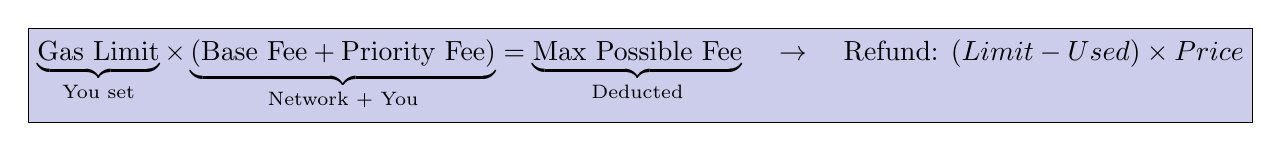
\begin{tikzpicture}[scale=0.9]
  % Formula box
  \node[draw, rectangle, fill=mllavender3, minimum width=12cm, minimum height=1.2cm] at (0,0) {
    $\underbrace{\text{Gas Limit}}_{\text{You set}} \times \underbrace{(\text{Base Fee} + \text{Priority Fee})}_{\text{Network + You}} = \underbrace{\text{Max Possible Fee}}_{\text{Deducted}}$ \quad $\rightarrow$ \quad Refund: $(Limit - Used) \times Price$
  };
\end{tikzpicture}
\end{center}

\bottomnote{Typical gas prices: 10-30 Gwei (low activity), 50-200 Gwei (high activity), 500+ Gwei (congestion)}
\end{frame}

% ==================== SLIDE 12: WHY GAS PREVENTS INFINITE LOOPS ====================
\begin{frame}[t,fragile]{Why Gas Prevents Infinite Loops}
\begin{columns}[T]
\column{0.48\textwidth}
\textbf{The Halting Problem}

\textit{Can we determine if a program will finish?}

\begin{itemize}
\item Mathematically proven impossible
\item Turing-complete = can loop forever
\item Ethereum allows Turing-completeness
\item Solution: Economic constraint (gas)
\end{itemize}

\vspace{0.5em}
\textbf{Without Gas}
\begin{itemize}
\item[\textcolor{mlred}{X}] Attacker deploys infinite loop
\item[\textcolor{mlred}{X}] All nodes stuck forever
\item[\textcolor{mlred}{X}] Network halts completely
\item[\textcolor{mlred}{X}] DoS attack succeeds
\end{itemize}

\column{0.48\textwidth}
\textbf{With Gas}
\begin{itemize}
\item[\textcolor{mlgreen}{\checkmark}] Each operation costs gas
\item[\textcolor{mlgreen}{\checkmark}] Gas limit caps execution
\item[\textcolor{mlgreen}{\checkmark}] Loop runs until gas exhausted
\item[\textcolor{mlgreen}{\checkmark}] Attacker pays for each iteration
\end{itemize}

\vspace{0.5em}
\textbf{Example: Malicious Loop}

\begin{lstlisting}[numbers=none, basicstyle=\ttfamily\tiny]
// This would be expensive!
while(true) {
  storage[i] = i;  // 20,000 gas each
  i++;
}
// At 20,000 gas/iteration:
// 100,000 gas = 5 iterations only!
\end{lstlisting}
\end{columns}

\bottomnote{Gas makes computation economically bounded; attackers must pay proportionally to damage attempted}
\end{frame}

% ==================== SECTION 3: SOLIDITY BASICS ====================
\section{Solidity Basics}

\begin{frame}[t]
\vfill
\centering
\begin{beamercolorbox}[sep=8pt,center]{title}
\usebeamerfont{title}\Large Section 3: Solidity Basics\par
\end{beamercolorbox}
\vfill
\small \textit{15 minutes}
\end{frame}

% ==================== SLIDE 13: WHAT IS SOLIDITY? ====================
\begin{frame}[t,fragile]{What is Solidity?}
\begin{columns}[T]
\column{0.48\textwidth}
\textbf{Solidity Overview}

\begin{itemize}
\item High-level language for smart contracts
\item Influenced by C++, Python, JavaScript
\item Compiles to EVM bytecode
\item Statically typed
\item Supports inheritance, libraries
\item Most popular smart contract language
\end{itemize}

\vspace{0.3em}
\begin{block}{Real-World Analogy}
A smart contract is like a \textbf{vending machine}. You put money in (send a transaction), press a button (call a function), and it automatically gives you the product (executes code). No human needed -- it's all automatic!
\end{block}

\vspace{0.3em}
\textbf{File Structure}
\begin{itemize}
\item \texttt{.sol} file extension
\item Pragma version declaration
\item Import statements
\item Contract definitions
\end{itemize}

\column{0.48\textwidth}
\textbf{Basic Contract Structure}

\begin{lstlisting}
// SPDX-License-Identifier: MIT
pragma solidity ^0.8.20;

contract MyContract {
    // State variables
    uint256 public value;

    // Constructor
    constructor() {
        value = 0;
    }

    // Functions
    function setValue(uint256 _v) public {
        value = _v;
    }
}
\end{lstlisting}
\end{columns}

\bottomnote{Always specify SPDX license and pragma version; use latest stable (0.8.x) for security features}
\end{frame}

% ==================== SLIDE 14: SOLIDITY DATA TYPES CHART ====================
\begin{frame}[t,fragile]{Solidity Data Types}
\begin{columns}[T]
\column{0.32\textwidth}
\textbf{Value Types}

\begin{tabular}{ll}
\texttt{bool} & true/false \\
\texttt{uint} & 0 to $2^{256}-1$ \\
\texttt{int} & $-2^{255}$ to $2^{255}-1$ \\
\texttt{address} & 20-byte value \\
\texttt{bytes32} & Fixed bytes \\
\end{tabular}

\vspace{0.5em}
\textbf{Sized Variants}
\begin{itemize}
\item \texttt{uint8} to \texttt{uint256}
\item \texttt{int8} to \texttt{int256}
\item \texttt{bytes1} to \texttt{bytes32}
\end{itemize}

\column{0.32\textwidth}
\textbf{Reference Types}

\begin{tabular}{ll}
\texttt{string} & UTF-8 text \\
\texttt{bytes} & Dynamic bytes \\
\texttt{array[]} & Dynamic array \\
\texttt{array[N]} & Fixed array \\
\texttt{struct} & Custom type \\
\end{tabular}

\vspace{0.5em}
\textbf{Data Locations}
\begin{itemize}
\item \texttt{storage} - persistent
\item \texttt{memory} - temporary
\item \texttt{calldata} - read-only
\end{itemize}

\column{0.32\textwidth}
\textbf{Special Types}

\begin{tabular}{ll}
\texttt{mapping} & Hash table \\
\texttt{enum} & Enumeration \\
\texttt{contract} & Contract ref \\
\end{tabular}

\vspace{0.5em}
\textbf{Mapping Example}
\begin{lstlisting}[numbers=none, basicstyle=\ttfamily\tiny]
// address -> balance
mapping(address => uint)
    public balances;

// Nested mapping
mapping(address =>
  mapping(address => uint))
    public allowance;
\end{lstlisting}
\end{columns}

\bottomnote{Mappings cannot be iterated; use arrays alongside if enumeration needed}
\end{frame}

% ==================== SLIDE 15: STATE VARIABLES ====================
\begin{frame}[t,fragile]{State Variables}
\begin{columns}[T]
\column{0.48\textwidth}
\textbf{What Are State Variables?}

\begin{itemize}
\item Permanently stored on blockchain
\item Defined at contract level
\item Persist between function calls
\item Cost gas to read/write (storage)
\item Form the contract's "memory"
\end{itemize}

\vspace{0.5em}
\textbf{Visibility Modifiers}
\begin{itemize}
\item \texttt{public} - auto getter, accessible
\item \texttt{private} - contract only
\item \texttt{internal} - contract + derived
\end{itemize}

\column{0.48\textwidth}
\textbf{State Variable Examples}

\begin{lstlisting}
contract Bank {
    // Simple state
    address public owner;
    uint256 public totalDeposits;

    // Mapping state
    mapping(address => uint256)
        private balances;

    // Array state
    address[] public depositors;

    // Struct state
    struct Account {
        uint256 balance;
        bool active;
    }
    mapping(address => Account)
        public accounts;
}
\end{lstlisting}
\end{columns}

\bottomnote{State variables live in storage slots; packing smaller types saves gas (e.g., uint128 + uint128 in one slot)}
\end{frame}

% ==================== SLIDE 16: FUNCTIONS AND VISIBILITY ====================
\begin{frame}[t,fragile]{Functions and Visibility}
\begin{columns}[T]
\column{0.48\textwidth}
\textbf{Function Visibility}

\begin{tabular}{ll}
\toprule
\textbf{Modifier} & \textbf{Access} \\
\midrule
\texttt{public} & Anyone, internally \\
\texttt{external} & Only from outside \\
\texttt{internal} & Contract + children \\
\texttt{private} & Contract only \\
\bottomrule
\end{tabular}

\vspace{0.5em}
\textbf{State Mutability}
\begin{itemize}
\item \texttt{view} - reads state, no modify
\item \texttt{pure} - no state access
\item \texttt{payable} - can receive ETH
\item (none) - can modify state
\end{itemize}

\column{0.48\textwidth}
\textbf{Function Syntax}

\begin{lstlisting}
contract Functions {
    uint256 public value;

    // State-changing
    function setValue(uint256 _v)
        public {
        value = _v;
    }

    // View function
    function getValue()
        public view returns (uint256) {
        return value;
    }

    // Pure function
    function add(uint a, uint b)
        public pure returns (uint) {
        return a + b;
    }
}
\end{lstlisting}
\end{columns}

\bottomnote{Use \texttt{external} over \texttt{public} when function only called externally (saves gas)}
\end{frame}

% ==================== SLIDE 17: EVENTS ====================
\begin{frame}[t,fragile]{Events: Logging on the Blockchain}
\begin{columns}[T]
\column{0.48\textwidth}
\textbf{What Are Events?}

\begin{itemize}
\item Logging mechanism for contracts
\item Stored in transaction logs (not state)
\item Cheaper than storage
\item Can be filtered and searched
\item Used by frontends/dApps
\end{itemize}

\vspace{0.5em}
\textbf{Use Cases}
\begin{itemize}
\item Track token transfers
\item Record important state changes
\item Notify external applications
\item Create audit trails
\end{itemize}

\column{0.48\textwidth}
\textbf{Event Syntax}

\begin{lstlisting}
contract Token {
    // Event declaration
    event Transfer(
        address indexed from,
        address indexed to,
        uint256 value
    );

    event Approval(
        address indexed owner,
        address indexed spender,
        uint256 value
    );

    function transfer(address to, uint v)
        public {
        // ... transfer logic ...
        emit Transfer(msg.sender, to, v);
    }
}
\end{lstlisting}

\textit{\small\texttt{indexed}: searchable (max 3)}
\end{columns}

\bottomnote{Events cost ~375 gas base + 375 per indexed topic + 8 per byte of data}
\end{frame}

% ==================== SLIDE 18: CODE - HELLOWORLD.SOL ====================
\begin{frame}[t,fragile]{Code Example: HelloWorld.sol}
\begin{columns}[T]
\column{0.48\textwidth}
\begin{lstlisting}
// SPDX-License-Identifier: MIT
pragma solidity ^0.8.20;

/// @title HelloWorld
/// @notice First smart contract
contract HelloWorld {
    // State variable
    string public message;

    // Event for message changes
    event MessageChanged(
        address indexed sender,
        string newMessage
    );

    // Constructor sets initial msg
    constructor(string memory _msg) {
        message = _msg;
    }

    // Update the message
    function setMessage(string memory _m)
        public {
        message = _m;
        emit MessageChanged(msg.sender, _m);
    }
}
\end{lstlisting}

\column{0.48\textwidth}
\textbf{Code Walkthrough}

\begin{enumerate}
\item \textbf{License \& Pragma}: Required headers
\item \textbf{Contract}: Named container for code
\item \textbf{State Variable}: \texttt{message} stored on-chain
\item \textbf{Event}: Log when message changes
\item \textbf{Constructor}: Runs once at deployment
\item \textbf{Function}: Changes state, emits event
\end{enumerate}

\vspace{0.5em}
\textbf{Key Observations}
\begin{itemize}
\item \texttt{public} auto-creates getter
\item \texttt{memory} for temp string storage
\item \texttt{msg.sender} = caller address
\item Constructor params set at deploy
\end{itemize}
\end{columns}

\bottomnote{This simple contract demonstrates state, events, constructor, and public functions}
\end{frame}

% ==================== SLIDE 19: CODE - SIMPLESTORAGE.SOL ====================
\begin{frame}[t,fragile]{Code Example: SimpleStorage.sol}
\begin{columns}[T]
\column{0.48\textwidth}
\begin{lstlisting}
// SPDX-License-Identifier: MIT
pragma solidity ^0.8.20;

/// @title SimpleStorage
/// @notice Store and retrieve values
contract SimpleStorage {
    // State
    uint256 private storedValue;
    address public owner;

    // Events
    event ValueStored(uint256 indexed val);

    // Constructor
    constructor() {
        owner = msg.sender;
        storedValue = 0;
    }

    // Store a value
    function store(uint256 _value) public {
        storedValue = _value;
        emit ValueStored(_value);
    }

    // Retrieve the value
    function retrieve()
        public view returns (uint256) {
        return storedValue;
    }
}
\end{lstlisting}

\column{0.48\textwidth}
\textbf{Key Concepts Demonstrated}

\begin{itemize}
\item \textbf{Private vs Public}:
  \begin{itemize}
  \item \texttt{storedValue} - no auto getter
  \item \texttt{owner} - has auto getter
  \end{itemize}
\item \textbf{Explicit Getter}: \texttt{retrieve()} function
\item \textbf{Owner Pattern}: Track deployer
\end{itemize}

\vspace{0.5em}
\textbf{Gas Costs}
\begin{itemize}
\item \texttt{store()}: ~43,000 gas (first write)
\item \texttt{store()}: ~26,000 gas (update)
\item \texttt{retrieve()}: FREE (view)
\end{itemize}

\vspace{0.5em}
\textbf{Why Free?}

View functions execute locally without transaction (no state change, no gas).
\end{columns}

\bottomnote{Pattern: Track owner in constructor for access control; retrieve() is a view (free)}
\end{frame}

% ==================== SLIDE 20: CONSTRUCTOR AND DEPLOYMENT ====================
\begin{frame}[t,fragile]{Constructor and Deployment}
\begin{columns}[T]
\column{0.48\textwidth}
\textbf{Constructor Characteristics}

\begin{itemize}
\item Runs \textbf{once} at deployment
\item Cannot be called again
\item Initializes state variables
\item Can receive parameters
\item Can receive ETH (\texttt{payable})
\end{itemize}

\vspace{0.5em}
\textbf{Constructor Patterns}

\begin{lstlisting}
constructor() {
    owner = msg.sender;  // Track deployer
}

constructor(uint256 _initial) {
    value = _initial;  // Parameterized
}

constructor() payable {
    // Can receive ETH at deploy
}
\end{lstlisting}

\column{0.48\textwidth}
\textbf{Deployment Process}

\begin{enumerate}
\item Compile Solidity to bytecode
\item Create deployment transaction
\item Include constructor args (ABI-encoded)
\item Send to null address (0x0)
\item EVM executes init code
\item Contract gets address
\item Runtime bytecode stored on-chain
\end{enumerate}

\vspace{0.5em}
\textbf{Contract Address}

$$\text{address} = \text{keccak256}(\text{sender}, \text{nonce})$$

\textit{Predictable! CREATE2 allows salt-based addresses.}
\end{columns}

\bottomnote{Deployment gas = base cost (32,000) + init code execution + runtime code storage (200 gas/byte)}
\end{frame}

% ==================== SLIDE 21: VIEW VS PURE FUNCTIONS ====================
\begin{frame}[t,fragile]{View vs Pure Functions}
\begin{columns}[T]
\column{0.48\textwidth}
\textbf{View Functions}

Read state but don't modify:

\begin{lstlisting}
uint256 public balance;

// Can read state
function getBalance()
    public view returns (uint256) {
    return balance;  // OK: reading
}

function getDoubleBalance()
    public view returns (uint256) {
    return balance * 2;  // OK
}

// ERROR: view cannot modify
function setBalance(uint _b)
    public view {
    balance = _b;  // COMPILE ERROR
}
\end{lstlisting}

\column{0.48\textwidth}
\textbf{Pure Functions}

No state access at all:

\begin{lstlisting}
// Pure: only uses parameters
function add(uint a, uint b)
    public pure returns (uint) {
    return a + b;  // OK
}

function hash(bytes memory data)
    public pure returns (bytes32) {
    return keccak256(data);  // OK
}

// ERROR: pure cannot read state
function pureError()
    public pure returns (uint) {
    return balance;  // COMPILE ERROR
}
\end{lstlisting}
\end{columns}

\vspace{0.5em}
\begin{center}
\begin{tabular}{lccc}
\toprule
& \textbf{Read State} & \textbf{Modify State} & \textbf{Cost (external call)} \\
\midrule
\texttt{view} & Yes & No & Free \\
\texttt{pure} & No & No & Free \\
(none) & Yes & Yes & Gas \\
\bottomrule
\end{tabular}
\end{center}

\bottomnote{Always use view/pure when possible; the compiler enforces these constraints}
\end{frame}

% ==================== SLIDE 22: MODIFIERS ====================
\begin{frame}[t,fragile]{Modifiers: Reusable Function Guards}
\begin{columns}[T]
\column{0.48\textwidth}
\textbf{What Are Modifiers?}

\begin{itemize}
\item Reusable code for function checks
\item Execute before/after function body
\item Common for access control
\item Use \texttt{\_} as function placeholder
\end{itemize}

\vspace{0.5em}
\textbf{Modifier Syntax}

\begin{lstlisting}
modifier onlyOwner() {
    require(
        msg.sender == owner,
        "Not owner"
    );
    _;  // Function body goes here
}

modifier nonReentrant() {
    require(!locked, "Reentrant");
    locked = true;
    _;  // Function executes
    locked = false;  // After function
}
\end{lstlisting}

\column{0.48\textwidth}
\textbf{Using Modifiers}

\begin{lstlisting}
contract Ownable {
    address public owner;
    bool private locked;

    constructor() {
        owner = msg.sender;
    }

    modifier onlyOwner() {
        require(msg.sender == owner);
        _;
    }

    // Only owner can call
    function withdraw()
        public onlyOwner {
        payable(owner).transfer(
            address(this).balance
        );
    }

    // Multiple modifiers
    function sensitive()
        public onlyOwner nonReentrant {
        // Protected code
    }
}
\end{lstlisting}
\end{columns}

\bottomnote{Modifiers reduce code duplication; OpenZeppelin provides battle-tested modifiers}
\end{frame}

% ==================== SECTION 4: DEPLOY & INTERACT ====================
\section{Deploy \& Interact}

\begin{frame}[t]
\vfill
\centering
\begin{beamercolorbox}[sep=8pt,center]{title}
\usebeamerfont{title}\Large Section 4: Deploy \& Interact\par
\end{beamercolorbox}
\vfill
\small \textit{10 minutes}
\end{frame}

% ==================== SLIDE 23: SMART CONTRACT LIFECYCLE CHART ====================
\begin{frame}[t]{Smart Contract Lifecycle}
\begin{center}
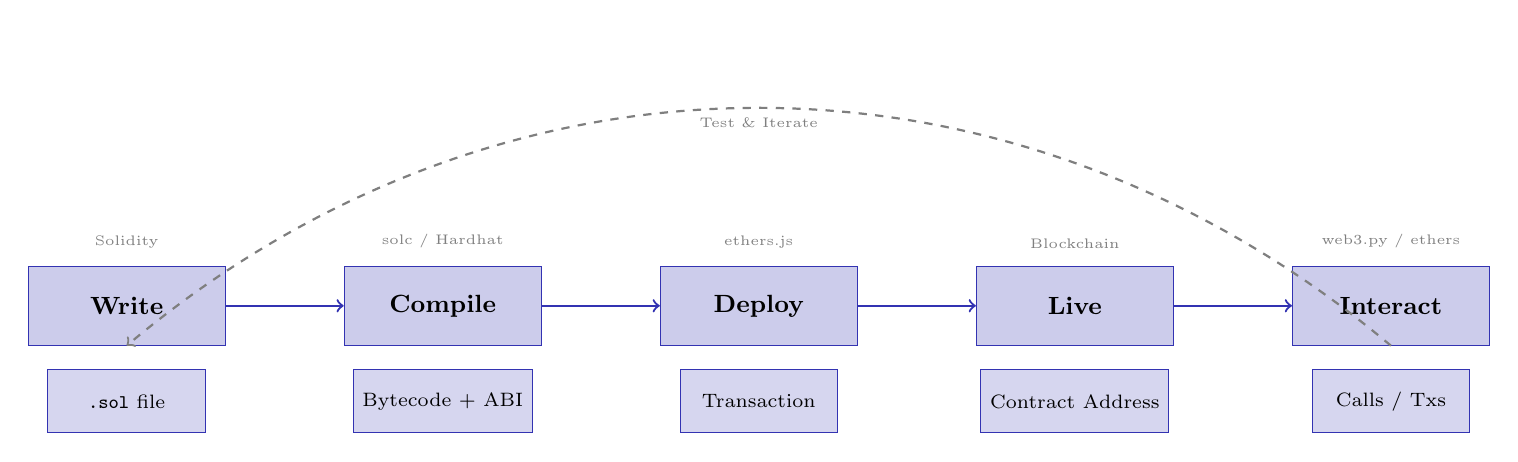
\begin{tikzpicture}[
  node distance=1.2cm,
  box/.style={rectangle, draw=mlpurple, fill=mllavender4, minimum width=2cm, minimum height=0.8cm, align=center, font=\scriptsize},
  bigbox/.style={rectangle, draw=mlpurple, fill=mllavender3, minimum width=2.5cm, minimum height=1cm, align=center, font=\small\bfseries},
  arrow/.style={->, thick, mlpurple}
]

% Development phase
\node[bigbox] (write) at (0,0) {Write};
\node[box, below=0.3cm of write] (sol) {\texttt{.sol} file};

\node[bigbox, right=1.5cm of write] (compile) {Compile};
\node[box, below=0.3cm of compile] (byte) {Bytecode + ABI};

\node[bigbox, right=1.5cm of compile] (deploy) {Deploy};
\node[box, below=0.3cm of deploy] (tx) {Transaction};

\node[bigbox, right=1.5cm of deploy] (live) {Live};
\node[box, below=0.3cm of live] (addr) {Contract Address};

\node[bigbox, right=1.5cm of live] (interact) {Interact};
\node[box, below=0.3cm of interact] (calls) {Calls / Txs};

% Arrows
\draw[arrow] (write) -- (compile);
\draw[arrow] (compile) -- (deploy);
\draw[arrow] (deploy) -- (live);
\draw[arrow] (live) -- (interact);

% Tools labels
\node[font=\tiny, text=mlgray, above=0.1cm of write] {Solidity};
\node[font=\tiny, text=mlgray, above=0.1cm of compile] {solc / Hardhat};
\node[font=\tiny, text=mlgray, above=0.1cm of deploy] {ethers.js};
\node[font=\tiny, text=mlgray, above=0.1cm of live] {Blockchain};
\node[font=\tiny, text=mlgray, above=0.1cm of interact] {web3.py / ethers};

% Feedback loop
\draw[arrow, dashed, mlgray] (interact.south) to[bend right=40] node[below, font=\tiny] {Test \& Iterate} (write.south);

\end{tikzpicture}
\end{center}

\vspace{0.5em}
\begin{columns}[T]
\column{0.32\textwidth}
\textbf{Development}
\begin{itemize}
\item Write Solidity code
\item Compile to bytecode
\item Generate ABI (interface)
\end{itemize}

\column{0.32\textwidth}
\textbf{Deployment}
\begin{itemize}
\item Send creation tx
\item Pay deployment gas
\item Get contract address
\end{itemize}

\column{0.32\textwidth}
\textbf{Interaction}
\begin{itemize}
\item Call view functions (free)
\item Send transactions (gas)
\item Emit/listen to events
\end{itemize}
\end{columns}

\bottomnote{Contracts are immutable once deployed; use proxy patterns for upgradeability}
\end{frame}

% ==================== SLIDE 24: DEVELOPMENT TOOLS - HARDHAT ====================
\begin{frame}[t,fragile]{Development Tools: Hardhat}
\begin{columns}[T]
\column{0.48\textwidth}
\textbf{What is Hardhat?}

Modern Ethereum development environment:

\begin{itemize}
\item Local blockchain network
\item Compilation and testing
\item Deployment scripts
\item Debugging with stack traces
\item Plugin ecosystem
\end{itemize}

\vspace{0.5em}
\textbf{Project Setup}

\begin{lstlisting}[style=javascript, numbers=none, basicstyle=\ttfamily\tiny]
# Initialize project
npm init -y
npm install --save-dev hardhat

# Create Hardhat project
npx hardhat init

# Project structure:
# contracts/   <- Solidity files
# scripts/     <- Deploy scripts
# test/        <- Test files
# hardhat.config.js
\end{lstlisting}

\column{0.48\textwidth}
\textbf{Common Commands}

\begin{lstlisting}[style=javascript, numbers=none, basicstyle=\ttfamily\tiny]
# Compile contracts
npx hardhat compile

# Run local blockchain
npx hardhat node

# Run tests
npx hardhat test

# Deploy to local network
npx hardhat run scripts/deploy.js
  --network localhost

# Deploy to testnet
npx hardhat run scripts/deploy.js
  --network sepolia
\end{lstlisting}

\vspace{0.5em}
\textbf{Alternatives}
\begin{itemize}
\item Foundry (Rust-based, fast)
\item Remix (browser IDE)
\item Truffle (legacy)
\end{itemize}
\end{columns}

\bottomnote{Hardhat provides console.log() in Solidity for debugging - invaluable during development}
\end{frame}

% ==================== SLIDE 25: LOCAL BLOCKCHAIN SETUP ====================
\begin{frame}[t,fragile]{Local Blockchain Setup}
\begin{columns}[T]
\column{0.48\textwidth}
\textbf{Hardhat Network}

Built-in local Ethereum network:

\begin{itemize}
\item Instant mining (no wait)
\item Pre-funded test accounts
\item Console.log support
\item Time manipulation
\item State snapshots
\end{itemize}

\vspace{0.5em}
\textbf{Start Local Node}

\begin{lstlisting}[style=javascript, numbers=none, basicstyle=\ttfamily\tiny]
$ npx hardhat node

Started HTTP and WebSocket JSON-RPC
server at http://127.0.0.1:8545/

Account #0: 0xf39Fd6e51aad88F...
Private Key: 0xac0974bec39a17e...
(10000 ETH)

Account #1: 0x70997970C51812d...
Private Key: 0x59c6995e998f97a...
(10000 ETH)
...
\end{lstlisting}

\column{0.48\textwidth}
\textbf{Network Configuration}

\begin{lstlisting}[style=javascript, numbers=none, basicstyle=\ttfamily\tiny]
// hardhat.config.js
module.exports = {
  solidity: "0.8.20",
  networks: {
    localhost: {
      url: "http://127.0.0.1:8545"
    },
    sepolia: {
      url: process.env.SEPOLIA_URL,
      accounts: [process.env.PRIVATE_KEY]
    },
    mainnet: {
      url: process.env.MAINNET_URL,
      accounts: [process.env.PRIVATE_KEY]
    }
  }
};
\end{lstlisting}

\vspace{0.5em}
\textbf{Test Networks}
\begin{itemize}
\item Sepolia - Ethereum testnet
\item Goerli - Being deprecated
\item Holesky - New testnet
\end{itemize}
\end{columns}

\bottomnote{Never use mainnet private keys in config files; use environment variables}
\end{frame}

% ==================== SLIDE 26: CODE - DEPLOYMENT SCRIPT ====================
\begin{frame}[t,fragile]{Code: Deployment Script}
\begin{columns}[T]
\column{0.48\textwidth}
\textbf{scripts/deploy.js}

\begin{lstlisting}[style=javascript]
const { ethers } = require("hardhat");

async function main() {
  // Get deployer account
  const [deployer] = await
    ethers.getSigners();

  console.log("Deploying with:",
    deployer.address);

  // Get contract factory
  const SimpleStorage = await
    ethers.getContractFactory(
      "SimpleStorage"
    );

  // Deploy contract
  const storage = await
    SimpleStorage.deploy();

  // Wait for deployment
  await storage.waitForDeployment();

  console.log("Deployed to:",
    await storage.getAddress());
}

main().catch(console.error);
\end{lstlisting}

\column{0.48\textwidth}
\textbf{Deployment with Constructor Args}

\begin{lstlisting}[style=javascript]
async function main() {
  const HelloWorld = await
    ethers.getContractFactory(
      "HelloWorld"
    );

  // Pass constructor argument
  const hello = await
    HelloWorld.deploy("Hello!");

  await hello.waitForDeployment();

  // Verify initial state
  const msg = await hello.message();
  console.log("Message:", msg);
}
\end{lstlisting}

\vspace{0.5em}
\textbf{Run Deployment}
\begin{lstlisting}[style=javascript, numbers=none, basicstyle=\ttfamily\tiny]
$ npx hardhat run scripts/deploy.js
Deploying with: 0xf39Fd6e51aad...
Deployed to: 0x5FbDB2315678...
\end{lstlisting}
\end{columns}

\bottomnote{ethers.js v6 uses getContractFactory() and waitForDeployment(); v5 used deployed()}
\end{frame}

% ==================== SLIDE 27: CALL VS TRANSACTION CHART ====================
\begin{frame}[t]{Call vs Transaction}
\begin{center}
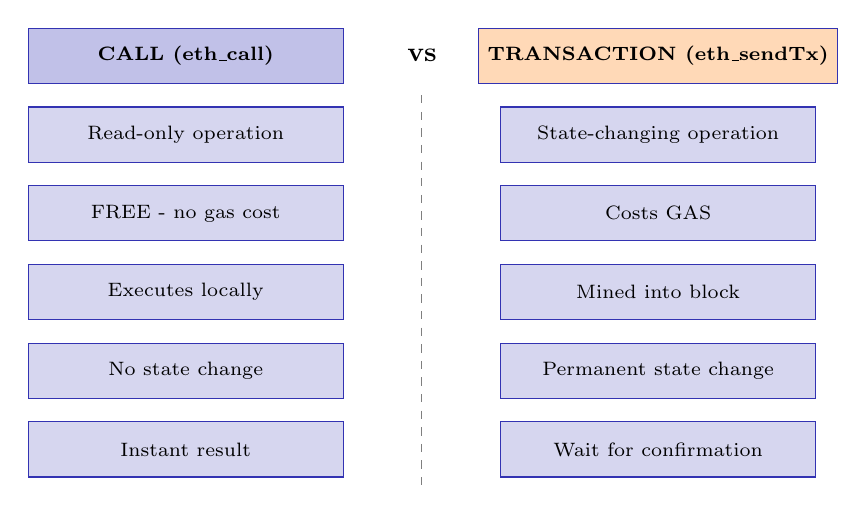
\begin{tikzpicture}[
  node distance=0.8cm,
  box/.style={rectangle, draw=mlpurple, fill=mllavender4, minimum width=4cm, minimum height=0.7cm, align=center, font=\scriptsize},
  arrow/.style={->, thick, mlpurple}
]

% Call side
\node[box, fill=mllavender2] (call) at (-3,2) {\textbf{CALL (eth\_call)}};
\node[box] (callread) at (-3,1) {Read-only operation};
\node[box] (callfree) at (-3,0) {FREE - no gas cost};
\node[box] (calllocal) at (-3,-1) {Executes locally};
\node[box] (callno) at (-3,-2) {No state change};
\node[box] (callsync) at (-3,-3) {Instant result};

% Transaction side
\node[box, fill=mlorange!30] (tx) at (3,2) {\textbf{TRANSACTION (eth\_sendTx)}};
\node[box] (txwrite) at (3,1) {State-changing operation};
\node[box] (txgas) at (3,0) {Costs GAS};
\node[box] (txmine) at (3,-1) {Mined into block};
\node[box] (txstate) at (3,-2) {Permanent state change};
\node[box] (txasync) at (3,-3) {Wait for confirmation};

% Middle comparison
\node at (0, 2) {\textbf{vs}};
\draw[dashed, mlgray] (0,1.5) -- (0,-3.5);

\end{tikzpicture}
\end{center}

\vspace{0.3em}
\begin{columns}[T]
\column{0.48\textwidth}
\textbf{Use CALL for:}
\begin{itemize}
\item \texttt{view} functions
\item \texttt{pure} functions
\item Reading balances, states
\item Simulating transactions
\end{itemize}

\column{0.48\textwidth}
\textbf{Use TRANSACTION for:}
\begin{itemize}
\item Modifying state variables
\item Transferring ETH/tokens
\item Emitting events
\item Any permanent change
\end{itemize}
\end{columns}

\bottomnote{Tip: Use eth\_call to simulate a transaction before sending to catch errors early}
\end{frame}

% ==================== SLIDE 28: CODE - PYTHON WEB3 INTERACTION ====================
\begin{frame}[t,fragile]{Code: Python web3 Interaction}
\begin{columns}[T]
\column{0.48\textwidth}
\textbf{Reading from Contract}

\begin{lstlisting}[style=python]
from web3 import Web3

# Connect to local node
w3 = Web3(Web3.HTTPProvider(
    'http://localhost:8545'
))

# Contract ABI (simplified)
abi = [
  {"name": "retrieve",
   "type": "function",
   "outputs": [{"type": "uint256"}],
   "stateMutability": "view"},
  {"name": "store",
   "type": "function",
   "inputs": [{"type": "uint256"}]}
]

# Contract instance
contract = w3.eth.contract(
    address='0x5FbDB2315678...',
    abi=abi
)

# Call view function (free)
value = contract.functions.retrieve()
    .call()
print(f"Stored value: {value}")
\end{lstlisting}

\column{0.48\textwidth}
\textbf{Writing to Contract}

\begin{lstlisting}[style=python]
# Your account
account = '0xf39Fd6e51aad88F...'
private_key = '0xac0974bec39a...'

# Build transaction
tx = contract.functions.store(42)
    .build_transaction({
        'from': account,
        'nonce': w3.eth.get_
            transaction_count(account),
        'gas': 100000,
        'gasPrice': w3.to_wei(
            '30', 'gwei')
    })

# Sign transaction
signed = w3.eth.account
    .sign_transaction(
        tx, private_key
    )

# Send and wait
tx_hash = w3.eth
    .send_raw_transaction(
        signed.raw_transaction
    )
receipt = w3.eth
    .wait_for_transaction_receipt(
        tx_hash
    )
print(f"Gas used: {receipt.gasUsed}")
\end{lstlisting}
\end{columns}

\bottomnote{Install: pip install web3; ABI is generated during compilation (artifacts/)}
\end{frame}

% ==================== SLIDE 29: TESTING YOUR CONTRACT ====================
\begin{frame}[t,fragile]{Testing Your Contract}
\begin{columns}[T]
\column{0.48\textwidth}
\textbf{test/SimpleStorage.test.js}

\begin{lstlisting}[style=javascript]
const { expect } = require("chai");
const { ethers } = require("hardhat");

describe("SimpleStorage", function() {
  let storage;
  let owner;

  beforeEach(async function() {
    [owner] = await ethers.getSigners();
    const Factory = await ethers
      .getContractFactory(
        "SimpleStorage"
      );
    storage = await Factory.deploy();
  });

  it("should store value",
    async function() {
    await storage.store(42);
    expect(await storage.retrieve())
      .to.equal(42n);
  });

  it("should emit event",
    async function() {
    await expect(storage.store(100))
      .to.emit(storage, "ValueStored")
      .withArgs(100);
  });
});
\end{lstlisting}

\column{0.48\textwidth}
\textbf{Run Tests}

\begin{lstlisting}[style=javascript, numbers=none, basicstyle=\ttfamily\tiny]
$ npx hardhat test

  SimpleStorage
    V should store value (45ms)
    V should emit event (38ms)

  2 passing (1s)
\end{lstlisting}

\vspace{0.5em}
\textbf{Testing Best Practices}

\begin{itemize}
\item Test all public functions
\item Test edge cases (0, max values)
\item Test access control (modifiers)
\item Test events are emitted
\item Test reverts with \texttt{revertedWith}
\item Use \texttt{beforeEach} for fresh state
\end{itemize}

\vspace{0.5em}
\textbf{Coverage}
\begin{lstlisting}[style=javascript, numbers=none, basicstyle=\ttfamily\tiny]
$ npx hardhat coverage
# Generates coverage report
\end{lstlisting}
\end{columns}

\bottomnote{Testing is crucial: bugs in deployed contracts can mean lost funds with no recourse}
\end{frame}

% ==================== SECTION 5: SUMMARY ====================
\section{Summary}

\begin{frame}[t]
\vfill
\centering
\begin{beamercolorbox}[sep=8pt,center]{title}
\usebeamerfont{title}\Large Section 5: Summary\par
\end{beamercolorbox}
\vfill
\small \textit{5 minutes}
\end{frame}

% ==================== SLIDE 30: KEY TAKEAWAYS ====================
\begin{frame}[t]{Key Takeaways}
\begin{columns}[T]
\column{0.48\textwidth}
\textbf{Ethereum Fundamentals}
\begin{itemize}
\item \checkmark Ethereum is a programmable blockchain
\item \checkmark EVM executes smart contracts identically on all nodes
\item \checkmark Two account types: EOA and Contract
\item \checkmark State is stored on-chain globally
\end{itemize}

\vspace{0.5em}
\textbf{Gas Mechanics}
\begin{itemize}
\item \checkmark Gas measures computation cost
\item \checkmark Prevents infinite loops and spam
\item \checkmark Fee = Gas Used $\times$ Gas Price
\item \checkmark Storage operations are most expensive
\end{itemize}

\column{0.48\textwidth}
\textbf{Solidity Essentials}
\begin{itemize}
\item \checkmark State variables provide persistent storage
\item \checkmark Functions: public, external, view, pure
\item \checkmark Events for logging (cheaper than storage)
\item \checkmark Modifiers for access control
\end{itemize}

\vspace{0.5em}
\textbf{Development Workflow}
\begin{itemize}
\item \checkmark Write $\rightarrow$ Compile $\rightarrow$ Deploy $\rightarrow$ Interact
\item \checkmark Use Hardhat for local development
\item \checkmark Test thoroughly before mainnet
\item \checkmark Call (free) vs Transaction (gas)
\end{itemize}
\end{columns}

\vspace{0.5em}
\begin{center}
\fbox{\parbox{0.9\textwidth}{\centering
\textbf{Golden Rule:} Smart contracts are immutable. Test extensively, audit code, and start with testnets before touching real ETH.
}}
\end{center}

\bottomnote{You now have the foundation to write and deploy your own smart contracts!}
\end{frame}

% ==================== SLIDE 31: NEXT LESSON PREVIEW ====================
\begin{frame}[t]{Next Lesson: Create Your Own Token}
\begin{columns}[T]
\column{0.48\textwidth}
\textbf{Lesson 4 Preview}

\begin{itemize}
\item ERC-20 Token Standard
\item Token interface and functions
\item Build a complete token contract
\item Deploy your own cryptocurrency
\item Transfer, approve, allowance pattern
\item Real-world token use cases
\end{itemize}

\vspace{0.5em}
\textbf{What You'll Build}
\begin{itemize}
\item Your own ERC-20 token
\item Token with custom features
\item Integration with DeFi concepts
\end{itemize}

\column{0.48\textwidth}
\textbf{Preparation}

\begin{enumerate}
\item Review today's Solidity basics
\item Practice with SimpleStorage
\item Set up Hardhat environment
\item Get Sepolia testnet ETH
\end{enumerate}

\vspace{0.5em}
\textbf{Resources}
\begin{itemize}
\item Solidity docs: docs.soliditylang.org
\item OpenZeppelin: openzeppelin.com/contracts
\item Hardhat: hardhat.org
\item Etherscan: etherscan.io
\end{itemize}

\vspace{0.5em}
\textit{Faucet: sepoliafaucet.com}
\end{columns}

\bottomnote{Lesson 4: From smart contracts to real tokens - the foundation of DeFi and NFTs}
\end{frame}

% ==================== SLIDE 32: QUESTIONS ====================
\begin{frame}[plain]
\vspace{3cm}
\begin{center}
{\Large Questions?}\\[2cm]
{\normalsize Thank you for your attention}\\[1cm]
{\small Lesson 3 of 4: Ethereum \& Smart Contracts}
\end{center}
\end{frame}

\end{document}
